\newcommand{\myfontsize}{11pt}


\documentclass[\myfontsize, letterpaper]{article}

\usepackage[margin=1.0in]{geometry}
\usepackage{color}
\usepackage{times}
\usepackage{amssymb}
\usepackage[labelfont=bf, font=scriptsize]{caption}
\usepackage{graphicx}
\usepackage{cite}
\usepackage{multicol}
\usepackage{amsmath}
\usepackage{setspace}
\usepackage{subfigure}


\usepackage{enumerate}

% TOGGLE MULTIPLE COLUMNS
\usepackage{etoolbox}
\newtoggle{cols}
\toggletrue{cols}
\togglefalse{cols}


\iftoggle{cols}{
    \newcommand{\myfigure}{figure*}
    \newcommand{\mytable}{table*}
}{
    \newcommand{\myfigure}{figure}
    \newcommand{\mytable}{table}
}



% linking
\usepackage{hyperref}

%TODO:
%apostrophes aren't showing up
%fix figures (use PS versions for high-res)
%fix paragraph indentation

% Add paragraph numbering, allows for numbering up to 5 levels deep.
% http://pleasemakeanote.blogspot.com/2010/06/how-to-activate-subsubsubsection-in.html
\setcounter{secnumdepth}{5}

% get rid of badness warnings in bibliography
% http://tex.stackexchange.com/questions/10924/underfull-hbox-in-bibliography
\usepackage{etoolbox}
\apptocmd{\sloppy}{\hbadness 10000\relax}{}{}

% adds line breaks after paragraph section headings
% http://tex.stackexchange.com/questions/32160/new-line-after-paragraph
\newcommand{\myparagraph}[1]{\paragraph{#1}\mbox{}\\[\myfontsize]}
\newcommand{\projectname}{VM2Docker}

\author{
    Eric Lubin\\
    \href{mailto:eblubin@mit.edu}{eblubin@mit.edu}
\\\\
    Thesis Advisor: \\
Martin Rinard, Professor MIT\\
    \href{mailto:rinard@csail.mit.edu}{rinard@lcs.mit.edu}
\\\\
Mentor:\\
Jim Yang, VMware \\
\href{mailto:jimyang@vmware.com}{jimyang@vmware.com}\\
}


\title{\projectname: Automating the Conversion from Virtual Machine to Docker Container \\[1\baselineskip] \Large{M.Eng Thesis Proposal}}

\begin{document}
\maketitle
\iftoggle{cols} {
    \begin{multicols}{2}
}
\doublespacing
\section{Introduction}
Historically, virtual machines have owned a staggering majority of the enterprise and devops marketplaces. Virtual machi TODOTODO
Recently, however, a relatively new framework called Docker hopes to redefine the industry. Making use of many recently added extensions to the linux kernel, Docker containers are a lightweight alternative to virtual machines that aim to streamline the developer workflow by creating shippable build environments without the bulk and performance degradation of running within a virtual machine.

Unlike virtual machines, containers share the kernel with the host and other containers running on that same host. For this reason, Docker containers only support linux-based operating systems and workflows, as opposed to the wider range of legacy and Windows-based operating systems that virtual machines promise to support.

For some, Docker containers may provide a cleaner, higher performing, alternative to virtual machines. However, the process of making the switch is currently by no means automatic. Docker requires the developer to manually decompose a virtual machine into a subset of required components: the base operating system, required libraries and other dependencies, and then the app or applications themselves that are running on the host. Converting one or a few virtual machines is feasible, but for enterprises with hundreds or thousands of VMs, a better solution is needed. For this reason, we would like to explore the feasibility of streamlining the conversion of a set of virtual machines to Docker containers in a highly automated and efficient manner. 

\section{Docker}

Docker is a platform that enables streamlined and automated building, shipping, and running of applications across a host of different environments. Each container provides a namespaced, isolated environment for execution. Docker exploits filesystem layering, as well as specific features of the linux kernel, to be able to run these environments in a lightweight manner that is faster and less expensive than running inside of a virtual machine.


talk about how containers can run one or many processes using something like supervisord.

\begin{figure}[h]
\centering
    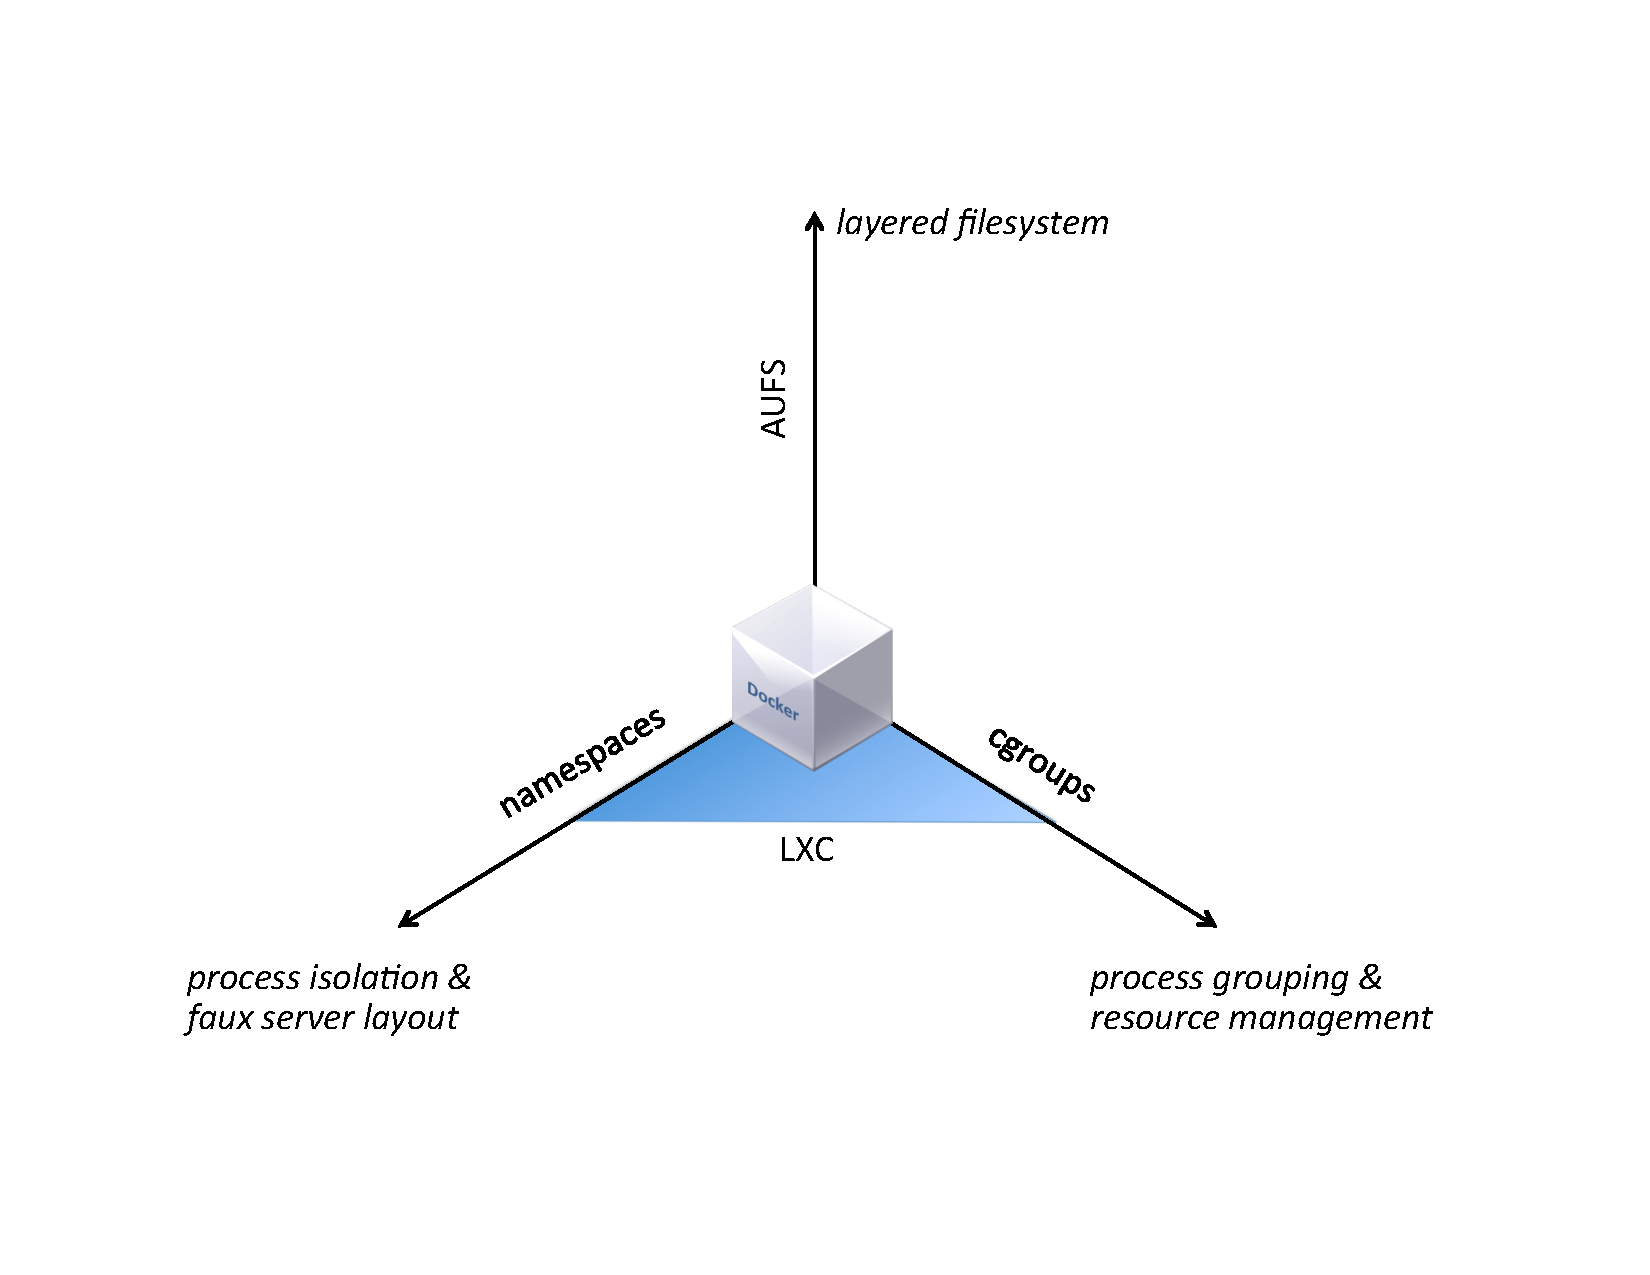
\includegraphics[width=1.0\textwidth]{docker.pdf}
    \caption{A graphic outlining the three fundamental components that make up the Docker framework. Namespace and cgroup support are provided by the LXC (LinuX Container) kernel extensions, and filesystem layering is provided by AUFS.}
\end{figure}

\subsection{Docker Engine}

\subsubsection{AUFS}
AUFS, Another Union FileSystem, is the primary means through which Docker achieves both storage savings and faster deployments of containers. Each image inherits from a sequence of other images, up to the base image, and represents the set or sequence of changes on the filesystem. This layering of filesystems and images accomplishes two main benefits. First, it allows for a high degree of storage savings. If two containers are running the same OS and share some libraries and dependencies, the majority of their filesystems will only be represented once on disk and are not duplicated. Second, when downloading and deploying a container, if a host already has previous layers of the filesystem on which a given container depends, it need only to download the incremental changes.

\subsubsection{namespaces}
Namespaces are the mechanism by which each Docker container is isolated from the host and other containers. There are many different namespaces that LXC supports, but probably the two most significant ones are the \texttt{pid} and \texttt{net} namespaces. The \texttt{pid} namespace is responsible for giving each container its own isolated environment for processes. A given container can only see and send signals to the processes that are running within the same container. In addition, the \texttt{net} namespace allows different containers to have what appears to be distinct network interfaces, thereby permitting two containers to simultaneously bind to the same port, for example \cite{lxc}.



\subsubsection{cgroups}
Cgroups, or control groups, are a feature on the linux kernel that provides resource limiting, in the form of memory or disk limits, as well as prioritization of CPU and disk throughput. These features are comparable to those offered by a virtual machine hypervisor to allocate a given amount of memory and CPU, network, and disk priority to a virtual machine.

\subsection{Docker Hub}

TODO LALALAL


\section{VMs vs Docker}

While it remains to be seen whether Docker poses an immediate threat to the virtual machine landscape, it is evident that virtual machines and containers are distinct products that aren't necessarily direct competitors and each cater to a slightly different audience.

Since Docker shares the kernel with the host, it only supports linux-based containers and immediately discards support for legacy enterprise software that might need a Windows environment to run.

Central to the distinction between container and virtual machine is the tradeoff between density and isolation. Virtual machines offer the strongest form of isolation, comparable to that offered by physically separated hosts. Containers, on the other hand, share the kernel with the host, and therefore provide a much larger attack surface through which an attacker might be able to compromise another container on the same host. 

By giving up isolation, unlike virtual machines which incur a performance overhead, containers achieve near native performance as compared to running directly on the host itself \cite{performance}. Furthermore, the density of containers on a given host can be much higher than that of VMs. 

\begin{figure}[h]
\centering
\subfigure[Docker Container]{%
  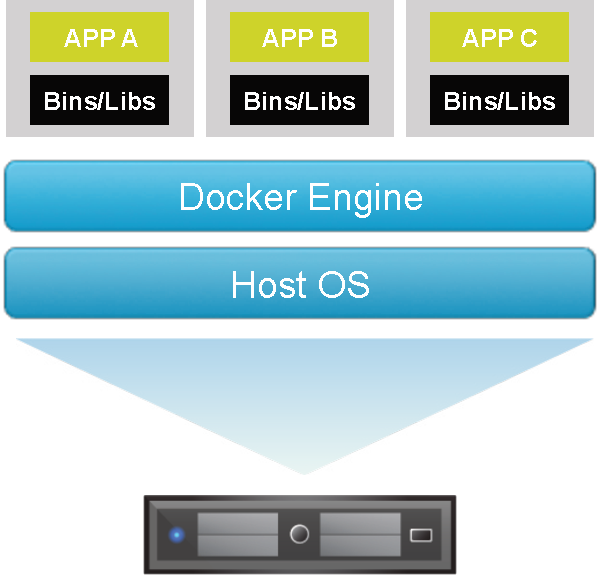
\includegraphics[width=.4\linewidth]{docker_h.pdf}
  \label{fig:sub1}}
\quad
\quad
\subfigure[Virtual Machine]{%
  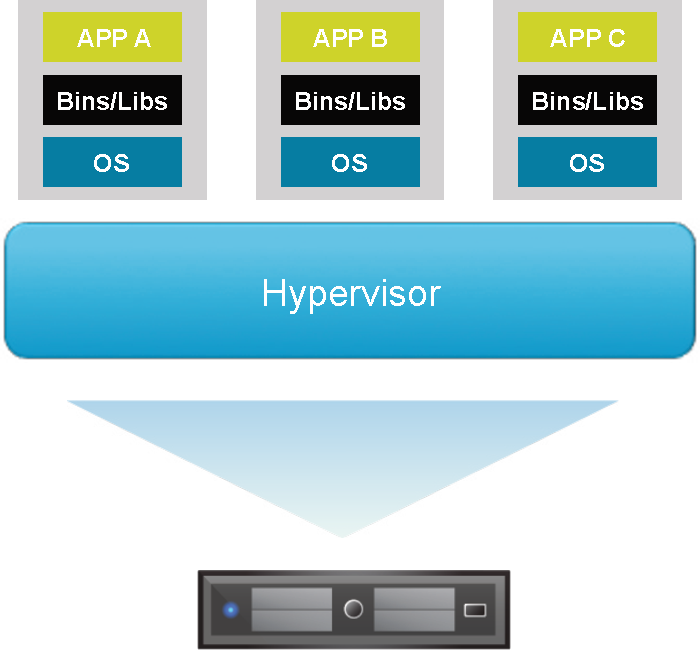
\includegraphics[width=.4\linewidth]{vm_h.pdf}
  \label{fig:sub2}}
\caption{A comparison of the components and isolation of virtual machines as compared to Docker containers. Each container consists of only an application and its dependencies and shares the underlying kernel with the host OS.}
\label{fig:test}
\end{figure}

Since Docker can run directly inside of a virtual machine, but not vice versa, there are interesting ways in which Docker and VMware might be able to work together in the future to offer a streamlined experience that captures the benefits of each. Multiple, trusted, containers running in the same VM, for example, could provide stronger isolation while still achieving the portability and deployment benefits that Docker containers provide.

\section{Previous Work}

The existing work in this field is fairly limited, and to the extent of our research there is no existing tool that attempts to automate the conversion from VM to container. Everything must be done manually.


\subsection{Filesystem}

Included with Docker is the import tool that has the following documentation:\\

\texttt{Usage: docker import URL|- [REPOSITORY[:TAG]]}

\texttt{Create an empty filesystem image and import the contents of the tarball (.tar, .tar.gz, .tgz, .bzip, .tar.xz, .txz) into it, then optionally tag it.} \\

Theoretically, this tool would permit us to create a tarball out of a full-fledged virtual machine and import it directly into Docker. However, doing so would completely abandon the notion of layering different filesystems together to construct an image, and the final Docker image would take up the same space as the original virtual machine. Furthermore, if multiple virtual machines were converted in this manner, even if they had the same underlying OS and distribution, their layers wouldn't share any of the same lineage. Thus, two docker images would take up the same amount of space as the original two VMs. 

As a result, Docker recommends that this tool be used only to create base images. In the Docker framework, base images are those images that do not have a parent and instead fully represent an entire OS on their own. Base images are used as starting points from which all other projects can inherit \cite{baseimage}. Base images should be made as small as possible and intuitively should only contain the necessary files to provide a fully-functioning OS. Packages can subsequently be installed on top of the base image depending on the desired function of the container. 

\subsection{Docker2VM}
Unlike the task of converting VMs to Docker, the converse is extremely straightforward. Since Docker can be run within a VM, one can simply run the same Docker container within a VM to obtain a Docker image that has been "converted" to a VM.

\section{\projectname}
To this effect, I propose an

 robust and fully extensible set of evolutionary game theory simulation tools. 

\subsection{Filesystem Layering}

talk more about the steps in this process with respect to base image detection and docker registry. public docker registry only has Ubuntu and CentOS base images, thus we will have to look for the existence of a base image, if it isn't there, announce the intention to make one, make the base image with debootstrap, then push that, then layer on top of the newly created base image. This will require the dependence on a local docker registry/index, which seems like a useful thing to have so that all of the VMs that are working together to convert to images can push the images they created to a private registry instead of just existing locally.


\begin{itemize}
\item Diff
\item Package management
\item Further space minimization via cache and kernel purging
\end{itemize}


IMPORTANT: also make another diagram outlining the "zipper-like" approach for undo-redo filesystem changes.

As an example, take the following table which shows the relative sizes of Ubuntu base images created for Docker, as compared to the sizes of Ubuntu VMs running corresponding distributions.

TABLE GOES HERE

In order to take advantage of Docker's layering filesystem, we propose that

\subsubsection{Verification}
need to make sure all of these undo/redo changes result in the same VM you started with.

TODO: with all of these filesystem transformations, we ran the container verification process to ensure that the resulting docker image, when built, represents a byte-for-byte equivalent filesystem as the original VM. This is essential to ensure correctness, and in all of our tests with various Ubuntu releases, verification was able to verify the results of our undo and redo transformations and exploitation of layering.


\subsection{Container Configuration}

On an abstract level, this encompasses a few major ideas:

\subsubsection{Mapping VM to Container}
1 to 1 or 1 to many????
outline some existing research in the area

configuration aspects:

consider moving this to the previous research section

\begin{itemize}
\item Resource allocation
\item Multi-container orchestration
\item Process specification - this can be done fairly easily on the host itself, by detecting what processes are open and the respective commands used to run them. Consider writing a wrapper script that converts a daemonized script to running in the foreground, without having to know the exact modifiers.
\item Port mapping
\end{itemize}


after having discussed the theoretically aspects, we can consider making such a configuration file tangible / compatible with existing frameworks:

\begin{itemize}
\item Fleet
\item Kubernetes
\item Fig
\end{itemize}

\subsection{Deployment}
As of this writing, the prototype of \projectname\ is a Python command-line program that is called by passing in the path to the root of the Virtual Machine filesystem. In effect, this is done by running the conversion script in an additional VM, which has mounted the VMDK of the VM to be converted. Since VMware software can itself mount VM disks (VMDK), this was the most straightforward method of obtaining access to the root filesystem of the VM. 

However, this method of conversion leaves much to be desired, as it requires each target VM to be manually mounted through the VMware user interface. The current prototype is therefore feasible for testing, but would quickly become unwieldy as the number of VMs approached hundreds or thousands.

As a longterm goal, \projectname\ should be able to be run on an entire virtual datacenter, and the virtual resources of a given VM should be able to be used in a distributed manner. In this way, the vSphere API could be used to streamline the simultaneous conversion of many VMs to docker images, without requiring any more additional compute resources than those already available and in use.

Similar to how existing tools are used to convert a physical host to VM, a self-contained executable could be downloaded and executed on a given host that would run the migration process from VM to container, or determine that the VM is not supported. Currently, the migration tool itself depends on the \texttt{rsync} utility, Python 2.7, the Python Docker client API, and an additional Python library called networkx. Additionally, the Docker command-line client is needed for importing base images from a tarball, since the Python library is largely inefficient.

Such an executable would need to install the required dependencies in an isolated part of the filesystem, then convert the VM to Docker using the existing tool while ignoring the dependencies needed to use the tool, and then push this new Docker image to a remote repository for subsequent access.

\section{Preliminary Results}

Thus far, we have focused on the filesystem aspect of the virtual machine conversion process. The results show a promising start to our goal of reducing the size of the resulting Docker containers by exploiting layering. For our data, we ran a prototype of the conversion script on six major releases of the Ubuntu distribution between 10.04 and the current 14.04 release. The scripts focus on just two of the aforementioned strategies for cutting down on the VM sizes:

\begin{enumerate}
\item Match up the VM with an existing base image and create a diff of the two
\item Detect existing installed packages (differs by distribution) and generate commands to reinstall them, rather than included these packages in the diff.
\end{enumerate}

We present the results of the first strategy, and then the two combined strategies, in the table and graphs below:

\subsection{Diff-Based Layering}
We match up each VM with its corresponding base image and then perform a diff using \texttt{rsync} to define the VM in terms of a set of additions, deletions, and changes applied to the base image. Table~\ref{table:diff} shows the space savings obtained by this process. Although the absolute reduction in space between the VM and the diff is relatively small, of interest is the amount of space saved relative to the base image. Since the diff is obtained relative to the base image, the maximal possible savings occurs if the VM represents only additions on the base image and the size reduction would be exactly equal to the size of the base image. We observe that the VMs are able to save between 35 and 72 \% of the size of the corresponding base image by taking advantage of layering and diffs. This space savings would manifest itself not only in a reduction of size of the container. In addition, assuming many containers inherit from the same image, it would also result in a reduction of time it takes for the container to be downloaded from a repository, a nontrivial performance benefit.

\begin{table}[h]
\centering
    \begin{tabular}{| c | c | c | c | c | c | c |}
    \hline
& \multicolumn{6}{|c|}{\bfseries Ubuntu Release} \\ \hline
    \bfseries Size (MB) & \itshape 10.04 & \itshape 12.04 & \itshape 12.10 & \itshape 13.04 & \itshape 13.10 & \itshape 14.04 \\ \hline
    \bfseries VM & 713 &  895 & 714 & 723 & 1006 & 1143\\ \hline
    \bfseries Base Image & 174 & 79 & 144 & 141 & 155 & 171  \\ \hline
    \bfseries Diff & 652 & 846 & 638 & 650 & 932 & 1020\\ \hline \hline
    \bfseries \% Saved & 35.1 & 62.0 & 52.8 & 51.8 & 47.7 & 71.9\\
    \hline
    \end{tabular}
\caption{The table above shows the space savings, compared to the original VM size, of converting to a Docker image that layers on top of the base image. The last row outlines the percentage of space saved, relative to the base image. 100\% would denote that the diff is exactly equal to the VM minus the base image.}
\label{table:diff}
\end{table}


Based on these results, we see that matching up a VM with a corresponding base image and calculating a diff alone begins to reap the benefits of Docker's layered container filesystem. In addition to this approach, the detection of installed packages available through the apt repository has further ability to drastically cut down on the weight and size of these VM-based containers.

\subsection{Package Management}

Another method of exploiting layering we used is based on the detection of the packages currently installed using the existing package manager. These packages, instead of being directly represented in the tarball of the diff, could be listed as a set of packages to be installed after the diff has been applied to the base image. As long as each package's uninstall and reinstall process are inverses and package configuration files are left as-is, the transformation would leave the resulting Docker container identical to the original.

Since most of the differences between the base image and the VM come in the form of packages, this package management strategy had the most significant impact on the resulting size of the diff. Of course, since the packages still need to be reinstalled on the container, the resulting container size is exactly the same. However, the package used to build this image is substantially smaller, which means the deployment time and portability of the package is improved.

The following table shows the reduction in diff sizes for various releases of Ubuntu, as obtained by applying the technique of package management and subsequent installation.

\begin{table}[h]
\centering
    \begin{tabular}{| c | c | c | c | c | c | c |}
    \hline
& \multicolumn{6}{|c|}{\bfseries Ubuntu Release} \\ \hline
    \bfseries Size of Diff (MB) & \itshape 10.04 & \itshape 12.04 & \itshape 12.10 & \itshape 13.04 & \itshape 13.10 & \itshape 14.04 \\ \hline
    \bfseries Before & 652 & 846 & 638 & 650 & 932 & 1020\\ \hline
    \bfseries After & 349 & 374 & 208 & 194 & 424 & 540  \\ \hline \hline
    \bfseries \% Reduction & 46.5 & 55.8 & 67.4 & 70.2 & 54.5 & 47.1\\
    \hline
    \end{tabular}
\caption{The table above shows the space savings, compared to the original diff size, of using a method of package management to further reduce the size of the diffs. The results reduced the size of the diff by between 66 and 70\%  and helped maximize portability of the resulting Docker build instructions.}
\label{table:diff}
\end{table}

Further experimentation will be done with various releases of other linux distributions such as CentOS, RedHat, Gentoo, BusyBox, Debian, and Fedora.



\section{Evaluation}

In addition to implementation, the results of the thesis can be evaluated in a number of objective and straightforward ways. 
\begin{itemize}
\item Compile filesystem data for image sizes and diff sizes for other linux distributions, such as CentOS, RedHat, and Gentoo
\item Attempt to quantify the time it takes to convert a VM to Docker container. This would largely vary depending on the VM, but mean and median statistics can be compiled.
\item Describe and quantify the tradeoff between decreasing image size and increasing build time of Docker container
\item Determine the efficiency of converting an entire virtual datacenter to Docker, capturing before and after space usage as well as performance metrics for standard tasks.
\item Establish a measure for the ability to convert VMs to containers without any user intervention, including what kinds of VMs can be seamlessly converted.
\end{itemize}

\section{Further Research}

Depending on if time permits, we would like to explore supporting the conversion of vApp to a set of containers. vApps are a logical set of Virtual Machines that work together to support a specific applications goals. This would likely map to a set of containers, where each container corresponds to a a given virtual machine. Just as the VMs are linked together through perhaps shared volumes and network communication, the containers' could be orchestrated to function in an analogous manner.


\begin{thebibliography}{99}
\bibitem{performance}
http://marceloneves.org/papers/pdp2013-containers.pdf

\bibitem{lxc}
http://blog.dotcloud.com/under-the-hood-linux-kernels-on-dotcloud-part
\bibitem{baseimage}
https://docs.docker.com/articles/baseimages/
\end{thebibliography}

\end{document}
